% ******** Приклад оформлення документа за ДСТУ 3008-95 ********
% ******************** автор: Тавров Д. Ю. *********************

% зазначаємо стильовий файл, який будемо використовувати
\documentclass{udstu}

% починаємо верстку документа
\begin{document}

% створимо титульний аркуш
% за допомогою спеціальної команди
% \maketitlepage{params},
% де params --- це розділені комами пари "параметр={значення}"
\maketitlepage{
% StudentName --- прізвище, ініціали студента
	StudentName={Скорденко Д. О.},
% StudentMale --- стать студента (true, якщо чоловік, false --- якщо жінка)
	StudentMale=true,
% StudentGroup --- група студента
	StudentGroup={КМ-01},
% Title --- назва
	Title={Звіт\\із лабораторної роботи №3\\із дисципліни \invcommas{Розподілені і хмарні обчислення}},
% SupervisorDegree --- науковий ступінь, учене звання керівника роботи
% якщо наукового ступеня немає, можна відповідний рядочок пропустити
	SupervisorDegree={доцент кафедри ПМА},
% SupervisorName --- прізвище, ініціали керівника роботи
	SupervisorName={Ліскін В. О.}
}

% створюємо зміст
\tableofcontents

% створюємо вступ
\intro

\paragraph{\textbf{Мета:}} порівняти інтегрування методом редукції за різної к-сті потоків.

Дослідний приклад:
\begin{equation*}
\begin{cases}
	f = \frac{1}{sin^2(2x)} \\
	a = 0 \\
	b = \pi/2
\end{cases}
\end{equation*}


% створюємо перший розділ роботи
\chapter{Основна частина}
\label{chap:1}

\paragraph{\textbf{Опис програми:}}

Для реалізації паралелізму буде використовуватись 'Rayon'.
Для порівняння швидоксті обчислень буде використовуватись 'Criterion'.

Порівняння буде проведено на різних к-стях відрізків $n \in [64, 1e5, 1e7]$,
та при різній к-сті потоків $nworkers \in [1,2,4,8]$


\chapter{Опис програми [Тестовий приклад]}
\label{chap:3}

\begin{figure}[!htp]
	\centering
	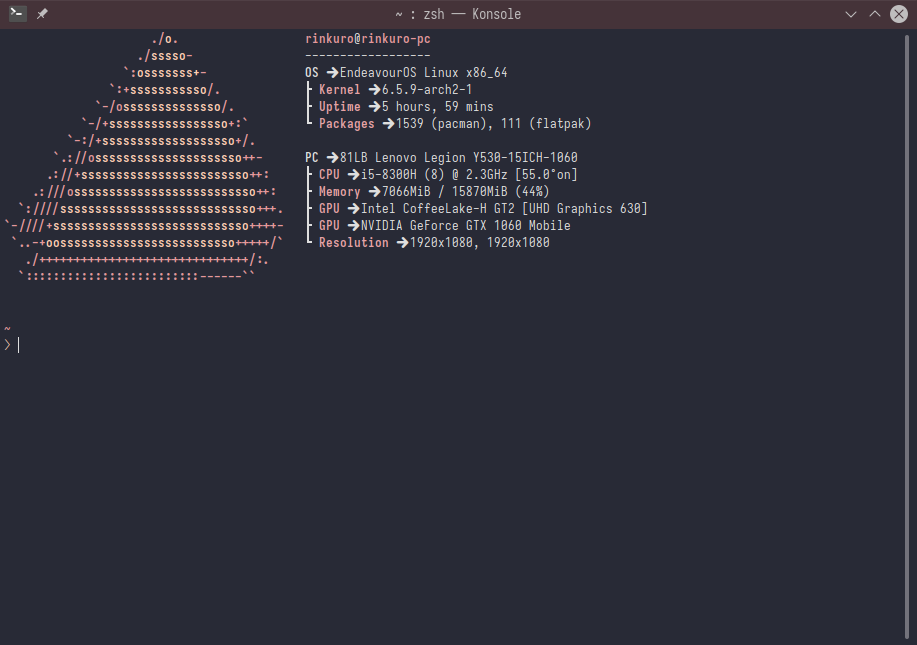
\includegraphics[scale=0.5]{PNG/system-specs.png}
	\caption{Характеристики системи}
	\label{fig:figure1}
\end{figure}

\begin{figure}[!htp]
	\centering
	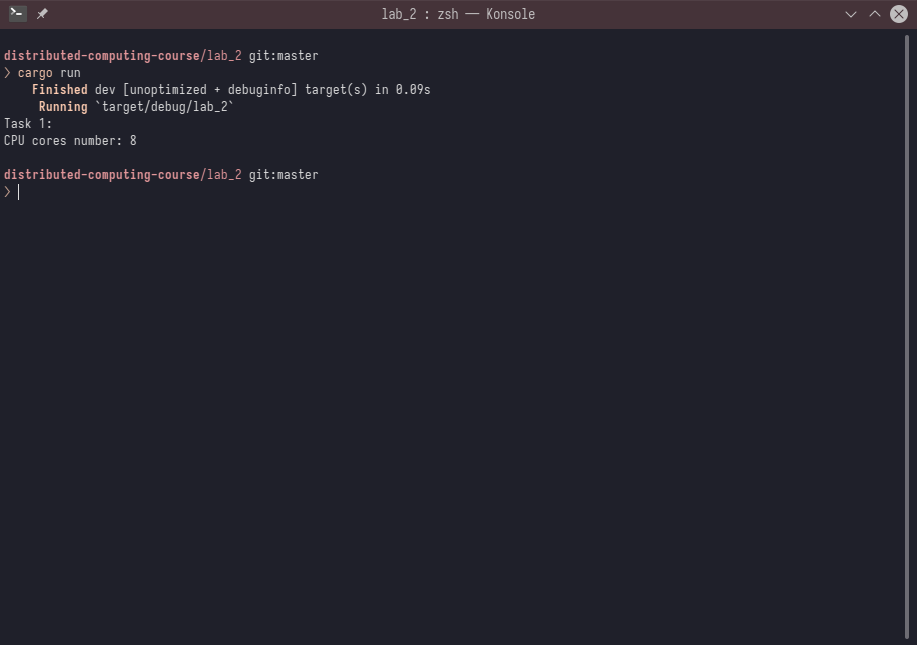
\includegraphics[scale=0.5]{PNG/thread-num-test.png}
	\caption{К-сть ядер процесора}
	\label{fig:figure1}
\end{figure}

\begin{center}
\captionof{table}{Порівняння швидкодії}
\resizebox{\textwidth}{!}{
\begin{tabular}{ | c | c | c | }
	\hline
	n & nworkers & time \\
	\hline
	64 & 1 & 8.0789 µs	8.2451 µs	8.4262 µs \\
	64 & 2 & 12.358 µs	12.759 µs	13.170 µs \\
	64 & 4 & 18.333 µs	18.765 µs	19.234 µs \\
	64 & 8 & 29.844 µs	30.635 µs	31.469 µs \\
	1e5 & 1 & 1.7601 ms	1.7908 ms	1.8307 ms \\
	1e5 & 2 & 912.96 µs	923.10 µs	934.10 µs \\
	1e5 & 4 & 542.83 µs	560.27 µs	578.18 µs \\
	1e5 & 8 & 484.52 µs	519.02 µs	575.76 µs \\
	1e7 & 1 & 165.89 ms	167.28 ms	168.80 ms \\
	1e7 & 2 & 84.522 ms	85.443 ms	86.488 ms \\
	1e7 & 4 & 43.958 ms	44.848 ms	45.868 ms \\
	1e7 & 8 & 36.668 ms	37.263 ms	37.933 ms \\
	\hline
\end{tabular}
}
\end{center}

% створюємо Висновки
\conclusions

На малих об'ємах обчислень збільшення к-сті потоків призводить до погіршення продуктивності.

На більших об'ємах збільшення потоків призводить до збільшення продуктивності,
однак після певної к-сті потоків ефект покращення продуктивності стає незначним.

\append{Код лістінги}

\paragraph{\textsc{*Примітка:}}
У код лістингах при копіюванні втрачається форматування (не копіюються пробіли).
Файли прикріплено до цього pdf (вкладка "прикріплені файли").

\captionof{listing}{integration.rs}
\embedfile[filespec=integration.rs]{../src/integration.rs}
\inputminted{rust}{../src/integration.rs}

\captionof{listing}{lib.rs}
\embedfile[filespec=lib.rs]{../src/lib.rs}
\inputminted{rust}{../src/lib.rs}

\captionof{listing}{main.rs}
\embedfile[filespec=main.rs]{../src/main.rs}
\inputminted{rust}{../src/main.rs}

\end{document}
